\section{Διαδίκτυο των Πραγμάτων}
\label{sec:theory_iot}

Το \textit{Διαδίκτυο των Πραγμάτων} (\textit{Internet of Things} ή \textit{IoT}) περιγράφει το δίκτυο φυσικών αντικειμένων - "πραγμάτων" - που είναι ενσωματωμένα με αισθητήρες, λογισμικό και άλλες τεχνολογίες με σκοπό τη σύνδεση και την ανταλλαγή δεδομένων με άλλες συσκευές και συστήματα μέσω του διαδικτύου. Αυτές οι συσκευές μπορεί να είναι συνηθισμένα οικιακά αντικείμενα, ή και εξελιγμένα βιομηχανική εργαλεία. Με περισσότερες από 7 δισεκατομμύρια συνδεδεμένες συσκευές IoT σήμερα, οι ειδικοί αναμένουν ότι ο αριθμός αυτός θα αυξηθεί σε 10 δισεκατομμύρια έως το 2020 και 22 δισεεκατομμύρια έως το 2025.

Μιας και δεν υπάρχει κάποιος συγκεκριμένος ορισμός για το IoT, αξίζει να παραθέσουμε τον ορισμό που έχει δοθεί και από το Ινστιτούτο Ηλεκτρολόγων και Ηλεκτρονικών Μηχανικών (IEEE) :

\say{Ένα δίκτυο αντικειμένων -το καθένα ενσωματωμένο με αισθητήρες- τα οποία είναι συνδεδεμένα στο διαδίκτυο} \cite{bib:chebudie_2014}

\subsection{Δομή του IoT}
\label{subsec:structure}

Η μονάδα υλικού σε ένα σύστημα IoT αποτελείται από τις ακόλουθες κατηγορίες:

\begin{itemize}
	\item Αισθητήρες/ενεργοποιητές
	\item Μονάδες επεξεργασίας
	\item Μονάδες αποθήκευσης
	\item Μονάδες επικοινωνίας
\end{itemize}

Έχοντας προσδιορίσει της κατηγορίες του υλικού, πρέπει να προσθέσουμε το λογισμικό, το ενδιάμεσο λογισμικό (middleware) και τα απαραίτητα πρωτόκολλα τα οποία παρέχουν τη δυνατότητα για να ενώσουμε όλα αυτά τα στοιχεία μεταξύ τους με σκοπό να συγκροτούν ένα πλήρως λειτουργικό σύστημα \cite{bib:chebudie_2014}.

Σε αυτήν την ενότητα, παρουσιάζεται η αρχιτεκτονική του IoT, το οποίο αποτελείται από τέσσερα επίπεδα (επίπεδο αίσθησης, επίπεδο δικτύου, επίπεδο επεξεργασίας δεδομένων, επίπεδο εφαρμογών) όπως φαίνεται και στο \autoref{fig:iot_layers} \cite{bib:kumar_2018}.

\begin{figure}[!ht]
	\centering
	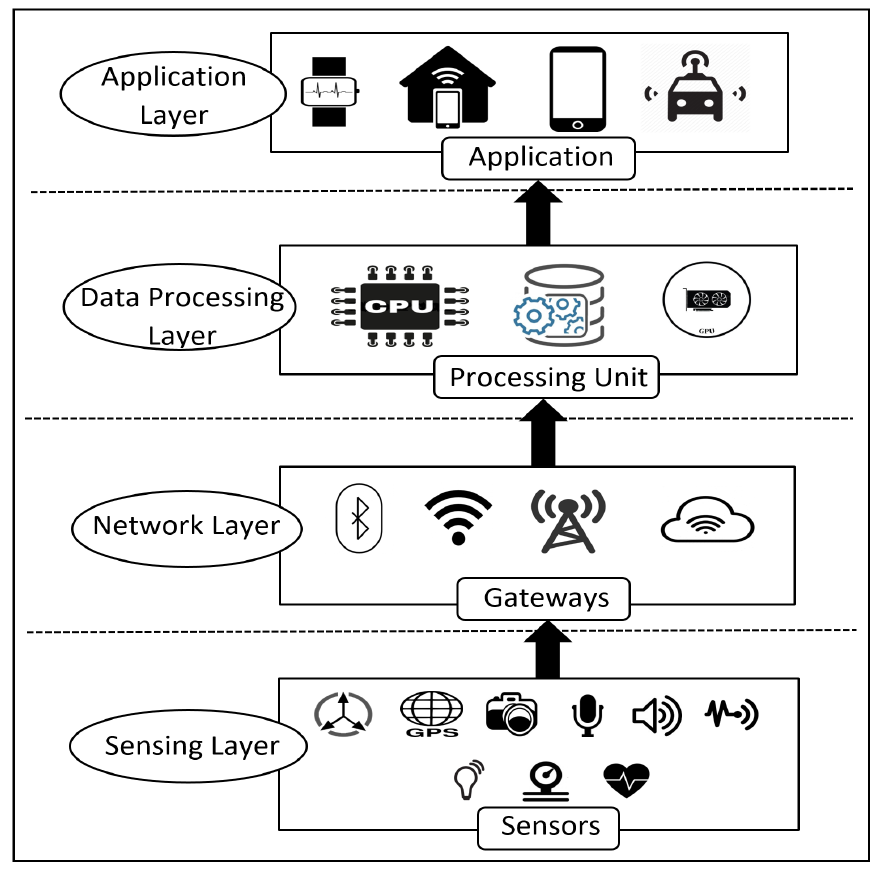
\includegraphics[width=0.6\textwidth]{./images/chapter2/iot_layers.png}
	\caption{Επίπεδα αρχιτεκτονικής του IoT.}
	\label{fig:iot_layers}
\end{figure}

\subsubsection{Επίπεδο Αίσθησης}
\label{subsubsec:sensing}

Ο κύριος σκοπός του επιπέδου αίσθησης είναι να ανιχνεύσει οποιαδήποτε φαινόμενα στο περιβάλλον των συσκευών και να λάβει δεδομένα από τον πραγματικό κόσμο. Το επίπεδο αυτό αποτελείται από διάφορους αισθητήρες, οι οποίοι ανήκουν στις ακόλουθες κατηγορίες:

\begin{enumerate}
	\item \textit{Αισθητήρες κίνησης:} Μετρούν την αλλαγή στην κίνηση καθώς και τον προσανατολισμό των συσκευών.
	\item \textit{Αισθητήρες περιβάλλοντος:} Αισθητήρες φωτός, πίεσης, θερμοκρασίας κ.α. αντιλαμβάνονται την αλλαγή σε περιβαλλοντικές παραμέτρους. 
	\item \textit{Αισθητήρες θέσης:} Είναι υπεύθυνοι για την εύρεση της φυσικής θέσης και τοποθεσίας της συσκευής (π.χ. μαγνητικοί σένσορες, GPS κ.α.).
\end{enumerate}

\subsubsection{Επίπεδο Δικτύου}
\label{subsubsec:network}

Το επίπεδο αυτό δρα ως κανάλι επικοινωνίας για τη μεταφορά δεδομένων, τα οποία συλλέχτηκαν στο επίπεδο αίσθησης, σε άλλες συνδεδεμένες συσκευές. Στις IoT συσκευές το επίπεδο δικτύου υλοποιείται με τη χρήση ποικίλων τεχνολογιών επικοινωνίας, όπως Wi-Fi, Bluetooth, Zegbee, Z-Wave, LoRa κ.α.

\subsubsection{Επίπεδο Επεξεργασίας Δεδομένων}
\label{subsubsec:data_proc}

Το επίπεδο επεξεργασίας δεδομένων αποτελείται από την κεντρική μονάδα επεξεργασίας των IoT συσκευών. Λαμβάνει τα δεδομένα από το επίπεδο αίσθησης, και τα αναλύει με σκοπό να πάρει αποφάσεις βάση του αποτελέσματος. Σε κάποιες IoT συσκευές, το επίπεδο αυτό αποθηκεύει το αποτέλεσμα προηγούμενων αναλύσεων με σκοπό τη βελτίωση της εμπειρίας χρήστη. Τέλος, μπορεί να μοιραστεί τα αποτελέσματα των αναλύσεων με άλλες συνδεδεμένες συσκευές μέσω του επιπέδου δικτύου.

\subsubsection{Επίπεδο Εφαρμογών}
\label{subsubsec:application}

Το τέταρτο και τελευταίο επίπεδο, υλοποιεί και παρουσιάζει τα αποτελέσματα του επιπέδο επεξεργασίας δεδομένων ώστε να εκτελέσει διάφορες λειτουργίες των IoT συσκευών.

\subsection{Πρωτόκολλο Επικοινωνίας Δεδομένων MQTT}
\label{subsec:mqtt}

Υπάρχουν διάφορα πρωτόκολλα επικοινωνίας δεδομένων τα οποία χρησιμοποιούνται στο IoT, ωστόσο στην παρούσα διπλωματική εργασία χρησιμοποιήθηκε το \textit{MQTT-SN} (\textit{Message Queuing Telemetry Transport for Sensor Networks}) το οποίο είναι μια διαφορετική έκδοση του MQTT\footnote{\url{https://mqtt.org/}}.

Ένα πολύ γνωστό παράδειγμα για επικοινωνία δεδομένων είναι το σύστημα \textit{"Publish/Subscribe"}, το οποίο θα μπορούσε να μεταφραστεί ως \textit{"Κοινοποίηση/Εγγραφή"}. Κατά τη λειτουργία ενός τέτοιου συστήματος, ο αποστολέας (publisher) δεν επικοινωνεί απευθείας με τον παραλήπτη (subscriber), αλλά κοινοποιεί τα μηνύματά του σε συγκεκριμένα \textit{τερματικά} (\textit{topics}), στα οποία ο παραλήπτης μπορεί να εγγραφεί και να λάβει τα μηνύματα που τους κοινοποιούνται. Υπεύθυνος για τη λήψη και διαμοιρασμό των μηνυμάτων, είναι ένας \textit{μεσολαβητής} (\textit{broker}).

Το πρότυπο αυτό μπορεί να υλοποιηθεί μέσω του πρωτοκόλλου MQTT. Το MQTT-SN που χρησιμοποιήθηκε στην εργασία, σχεδιάστηκε ώστε να είναι όσο το δυνατότερο όμοιο με το MQTT, αλλά είναι προσαρμοσμένο στις ιδιαιτερότητες ενός ασύρματου περιβάλλοντος επικοινωνίας, όπως είναι το χαμηλό εύρος ζώνης (bandwidth), οι υψηλές αποτυχίες συνδέσμων, το μικρό μήκος μηνύματος κ.α.